\chapter{ Констукторский раздел}
\label{cha:design}

В данном разделе мы рассмотрим схемы алгоритмов сортировки.

На рис. \ref{d:ref1} представлена схема алгоритма сортировки пузырьком.

\begin{figure}[ht!]
	\centering{
		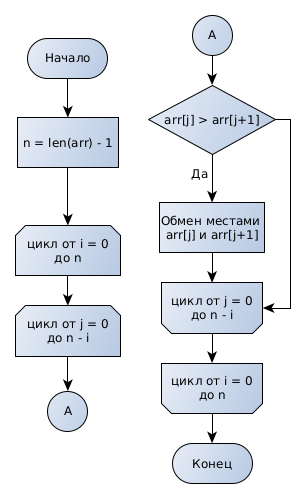
\includegraphics[width=0.5\textwidth]{img/unnamed0.png}
		\caption{Схема алгоритма сортировки пузырьком}
		\label{d:ref1}}
\end{figure}

На рис. \ref{d:ref2} представлена схема алгоритма сортировки вставками.

\begin{figure}[ht!]
	\centering{
		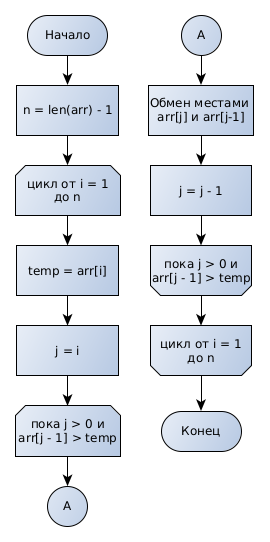
\includegraphics[width=0.5\textwidth]{img/unnamed1.png}
		\caption{Схема алгоритма сортировки вставками}
		\label{d:ref2}}
\end{figure}

На рис. \ref{d:ref3} представлена схема алгоритма quicksort.

\begin{figure}[ht!]
	\centering{
		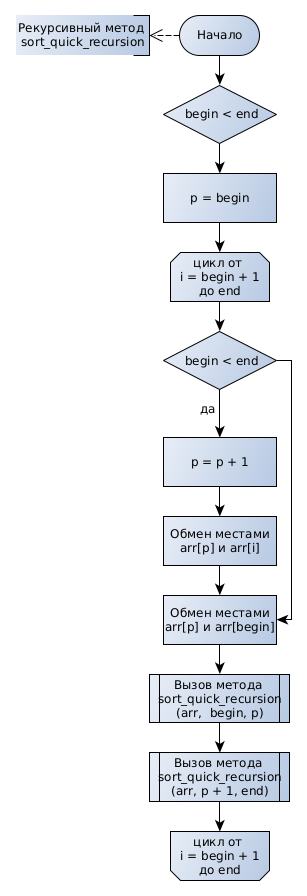
\includegraphics[width=0.5\textwidth]{img/unnamed2.png}
		\caption{Схема алгоритма сортировки quicksort}
		\label{d:ref3}}
\end{figure}


\section{Вывод}

В данном разделе были рассмотрены схемы (рис. \ref{d:ref1} - \ref{d:ref3}) алгоритмов сортировки.






